\chapter{Fully-connected models}
\label{chap:fully_connected_models}

\begin{supportbox}{About this chapter}
Standard programming is done by concatenating together the proper primitive operations. In this chapter we show that we can do something similar for differentiable models, by composing a sequence of so-called \textit{fully-connected layers}. For historical reasons, these models are also known as multilayer perceptrons (MLPs). MLPs are built by interleaving linear blocks (similar to Chapter \ref{chap:linear_models}) with non-linear functions, sometimes called \textit{activation functions}.
\end{supportbox}

\section{The limitations of linear models}

Linear models are fundamentally limited, in the sense that by definition they cannot model non-linear relationships across features. As an example, consider two input vectors $\mathbf{x}$ and $\mathbf{x}^\prime$, which are identical except for a single feature indexed by $j$:
%
$$
x_i^\prime=\begin{cases} x_i & \text{ if } i \neq j \\ 2x_i & \text{ otherwise } \end{cases}
$$
%
For example, this can represent two clients of a bank, which are identical in all aspects except for their income, with $\mathbf{x}^\prime$ having double the income of $\mathbf{x}$. If $f$ is a linear model (with no bias) we have:

\vspace{1em}
\begin{equation*}
f(\mathbf{x}^\prime) = \eqnmarkbox[drawred]{node}{f(\mathbf{x})} + \eqnmarkbox[drawblue]{node2}{w_jx_j}
\end{equation*}
\annotate[yshift=1em]{above,left}{node}{Original output}
\annotate[yshift=1em]{above,right}{node2}{Change induced by $x_j^\prime = 2x_j$}

Hence, the only consequence of the change in input is a small linear change of output dictated by $w_j$. Assume we are scoring the users, we may wish to model relationships such as “\textit{an income of 1500 is low, except if the age < 30}”.\footnote{You probably shouldn't do credit scoring with machine learning anyways.} Clearly, this cannot be done with a linear model due to the analysis above. 

The prototypical example of this is the XOR dataset, a two-valued dataset where each feature can only take values in $\left\{0, 1\right\}$. Hence, the entire dataset is given by only 4 possibilities:
%
$$
f([0,0])=0 \;,\; f([0,1])=1\;,\;f([1,0])=1\;,\;f([1,1])=0
$$
%
where the output is positive whenever \textit{only one} of the two inputs is positive. Despite its simplicity, this is also \textbf{non-linearly separable}, and cannot be solved with 100\% accuracy by a linear model - see Figure \ref{fig:xor} for a visualization.

\begin{SCfigure}
    \centering
    \hspace{1em}\includegraphics[width=0.5\textwidth]{images/XOR.pdf}
    \caption{Illustration of the XOR dataset: green squares are values of one class, red circles are values of another class. No linear model can separate them perfectly (putting all squares on one side and all circles on the other side of the decision boundary). We say that the dataset is not \textbf{linearly separable}.}
    \label{fig:xor}
\end{SCfigure}


\section{Composition and hidden layers}

\addclock A powerful idea in programming is decomposition, i.e., breaking down a problem into its constituent parts recursively, until each part can be expressed in simple, manageable operations. Something similar can be achieved in our case by imagining that our model $f$ is, in fact, the composition of two trainable operations:

$$
f(\mathbf{x})=(f_2 \circ f_1)(\mathbf{x})
$$

where $f_2 \circ f_1$ is the composition of the two functions: $(f_2 \circ f_1)(\mathbf{x}) = f_2(f_1(\mathbf{x}))$, and we assume that each function instantiates its own set of trainable parameters. We can keep subdividing the computations:

$$
f(\mathbf{x})=(f_l\circ f_{l-1}\circ \cdots\circ f_2\circ f_1)(\mathbf{x})
$$

where we now have a total of $l$ functions that are being composed. Note that as long as each $f_i$ does not change the “type” of its input data, we can chain together as many of these transformations as we want, and each one will add its own set of trainable parameters. 

For example, in our case the input $\mathbf{x}$ is a vector, hence any vector-to-vector operation (e.g., a matrix multiplication $f_i(\mathbf{x}) = \mathbf{W}\mathbf{x})$ can be combined together an endless number of times. However, some care must be taken. Suppose we chain together two different linear projections:
%
\begin{gather}
\mathbf{h} = f_1(\mathbf{x}) = \mathbf{W}_1\mathbf{x} +\mathbf{b}_1 \\y=f_2(\mathbf{h})=\mathbf{w}^\top_2\mathbf{h} + b_2
\end{gather}

It is easy to show that the two projections “collapse” into a single one:

$$
y = \underbrace{(\mathbf{w}^\top_2\mathbf{W}_1)}_{\triangleq\;\mathbf{A}}\mathbf{x} + \underbrace{(\mathbf{w}_2^\top\mathbf{b}_1 + b_2)}_{\triangleq \;\mathbf{c}} = \mathbf{A}\mathbf{x}+\mathbf{c}
$$
%
The idea of \textbf{fully-connected} (FC) models, also known as \textbf{multi-layer perceptrons} (MLPs) for historical reasons, is to insert a simple elementwise non-linearity $\phi : \mathbb{R} \rightarrow \mathbb{R}$ in-between projections to avoid the collapse:

\vspace{0.5em}
\begin{equation}
\mathbf{h} = f_1(\mathbf{x}) = \eqnmarkbox[drawred]{node}{\phi}\left(\mathbf{W}_1\mathbf{x} +\mathbf{b}_1\right)
\label{eq:mlps_single_hidden_layer_1}
\end{equation}%
\annotate[yshift=0.7em]{above,right}{node}{Element-wise non-linearity}
%
\begin{equation}
y=f_2(\mathbf{h})=\mathbf{w}^\top_2\mathbf{h} + b_2
\label{eq:mlps_single_hidden_layer_2}
\end{equation}

The second block can be linear, as in \eqref{eq:mlps_single_hidden_layer_2}, or it can be wrapped into another non-linearity depending on the task (e.g., a softmax function for classification). The function $\phi$ can be any non-linearity, e.g., a polynomial, a square-root, or the sigmoid function $\sigma$. As we will see in the next chapter, choosing it has a strong effect on the gradients of the model and, consequently, on optimization, and the challenge is to select a $\phi$ which is “non-linear enough” to prevent the collapse while staying as close as possible to the identity in its derivative. A good default choice is the so-called \textbf{rectified linear unit} (ReLU). 

\begin{definition}[Rectified linear unit] \addbottle
The \textbf{rectified linear unit} (ReLU) is defined elementwise as:
%
\begin{equation}
\textnormal{ReLU}(s)=\max(0,s)
\label{eq:relu}
\end{equation}
\end{definition}

We will have a lot more to say on the ReLU in the next chapter. With the addition of $\phi$, we can now chain as many transformations as we want:

\begin{equation}
y = \mathbf{w}_l^\top\phi\left( \mathbf{W}_{l-1}\left(\phi\left( \mathbf{W}_{l-2}\phi\left(\cdots\right)+\mathbf{b}_{l-2} \right)\right)+\mathbf{b}_{l-1} \right) + b_l
\label{eq:mlps_multiple_hidden_layer}
\end{equation}

In the rest of the chapter we focus on analyzing training and approximation properties of this class of models. First, however, a brief digression on naming conventions.

\subsection*{On the terminology used in differentiable models}

As we already mentioned, neural networks have a long history and a long baggage of terminology, which we briefly summarize here. Each $f_i$ is called a \textbf{layer} of the model, with $f_l$ being the \textbf{output layer}, $f_{i}, i=1,\ldots,l-1$ the \textbf{hidden layers} and, with a bit of notational overloading, $\mathbf{x}$ being the \textbf{input layer}. With this terminology, we can restate the definition of the \textbf{fully-connected layer} in batched form below.

\begin{definition}[Fully-connected layer] \addbottle
For a batch of $n$ vectors, each of size $c$, represented as a matrix $\mathbf{X} \sim (n,c)$, a \textbf{fully-connected} (FC) layer is defined as:
%
\begin{equation}
\textnormal{FC}(\mathbf{X}) = \phi\left(\mathbf{X}\mathbf{W} + \mathbf{b}\right)
\label{eq:fully_connected_layer}
\end{equation}
%
The parameters of the layer are the matrix $\mathbf{W} \sim (c^\prime,c)$ and the bias vector $\mathbf{b} \sim (c^\prime)$, for a total of $(c^\prime+1)c$ parameters (assuming $\phi$ does not have parameters). Its hyper-parameters are the width $c^\prime$ and the non-linearity $\phi$.
\end{definition}

The outputs $f_i(\mathbf{x})$ are called the \textbf{activations} of the layer, where we can sometimes distinguish between the \textbf{pre-activation} and the \textbf{post-activation} (before and after the non-linearity). The non-linearity $\phi$ itself can be called the \textbf{activation function}. Each output of $f_i$ is called a \textbf{neuron}. Although much of this terminology is outdated, it is still pervasive and we will use it when needed.

The size of the each layer (the shape of the output) is an hyperparameter that can be selected by the user, as it only influences the input shape of the next layer, which is known as the \textbf{width} of the layer. For a large number of  layers, the number of hyperparameters grows linearly and their selection becomes a combinatorial task. We will return on this point in Chapter \ref{chap:deep_cnns}, when we discuss the design of models with dozens (or hundreds) of layers.

\begin{mypy}{The FC layer in \eqref{eq:fully_connected_layer} implemented as an object in PyTorch. We require a special syntax to differentiate trainable parameters, such as $\mathbf{W}$, from other non-trainable tensors: in PyTorch, this is obtained by wrapping the tensors in a {\footnotesize\mintinline{python}{Parameter}} object. PyTorch also has its collection of layers in {\footnotesize\mintinline{python}{torch.nn}}, including the FC layer (implemented as {\footnotesize\mintinline{python}{torch.nn.Linear}}).}{code:fully_connected_layer}
class FullyConnectedLayer(nn.Module):
  def __init__(self, c: int, cprime: int):
    super().__init__()
    # Initialize the parameters
    self.W = nn.Parameter(torch.randn(c, cprime))
    self.b = nn.Parameter(torch.randn(1, cprime))

  def forward(self, x):
    return relu(x @ self.W + self.b)
\end{mypy}

The layer concept is also widespread in common frameworks. A layer such as \eqref{eq:fully_connected_layer} can be defined as an object having two functions: an initialization function that randomly initializes all parameters of the model based on the selected hyper-parameters, and a call function that provides the output of the layer itself. See Box \ref{code:fully_connected_layer} for an example. Then, a model can be defined by chaining together instances of such  layers. For example, in PyTorch this can be achieved by the {\footnotesize\mintinline{python}{Sequential}} object:

\vspace{1em}
{\begin{center}\footnotesize
\begin{minted}{python}
model = nn.Sequential(
    FullyConnectedLayer(3, 5), 
    FullyConnectedLayer(5, 4)
)
\end{minted}
\end{center}}
 
Note that from the point of view of their input-output signature, there is no great difference between a layer as defined in Box \ref{code:fully_connected_layer} and a model as defined above, and we could equivalently use \mintinline{python}{model} as a layer of a larger one. This compositionality is a defining characteristic of differentiable models.

\subsection{Approximation properties of MLPs} \addteacup

Training MLPs proceeds similarly to what we discussed for linear models. For example, for a regression task, we can minimize the mean-squared error:
%
$$
\underset{\left\{\mathbf{W}_k, \mathbf{b}_k\right\}_{k=1}^l}{\min} \;\; \frac{1}{n}\sum_{i} \left(y_i - f(\mathbf{x}_i)\right)^2
$$
%
where the minimization is now done on all parameters of the model simultaneously. We will see in the next lecture a general procedure to compute gradients in this case. 

For now, we note that the main difference with respect to having a linear model is that adding an hidden layer makes the overall optimization problem non-convex, with multiple local optima depending on the initialization of the model. This is an important aspect historically, as alternative approaches to supervised learning (e.g., support vector machines \cite{hofmann2008kernel}) provide non-linear models while remaining convex. However, the results of the last decade show that highly non-convex models can achieve significantly good performance in many tasks.\footnote{The reason differentiable models generalize so well is an interesting, open research question, to which we return in Chapter \ref{chap:deep_cnns}. Existing explanations range from an implicit bias of (stochastic) gradient descent \cite{pesme2021implicit} to intrinsic properties of the architectures themselves \cite{arpit2017closer,teney2024neural}.}

From a theoretical perspective, we can ask what is the significance of having added hidden layers, i.e., if linear models can only solve tasks which are linearly separable, what is instead the class of functions that can be approximated by adding hidden layers? As it turns out, having a single hidden layer is enough to have \textbf{universal approximation} capabilities. A seminal result in this sense was proved by G. Cybenko in 1989 \cite{cybenko1989approximation}.

\begin{theorem}[Universal approximation of MLPs \cite{cybenko1989approximation}]
Given a continuous function $g: \mathbb{R}^d \rightarrow \mathbb{R}$, we can always find a model $f(\mathbf{x})$ of the form \eqref{eq:mlps_single_hidden_layer_1}-\eqref{eq:mlps_single_hidden_layer_2} (an MLP with a single hidden layer) and sigmoid activation functions, such that for any $\varepsilon > 0$:
%
$$
\lvert f(\mathbf{x}) - g(\mathbf{x})\rvert\le\varepsilon \;,\;\forall \mathbf{x}
$$
%
where the result holds over a compact domain. Stated differently, one-hidden-layer MLPs are “dense” in the space of continuous functions.
\end{theorem}

The beauty of this theorem should not distract from the fact that this is purely a theoretical construct, that makes use of the fact that the width of the hidden layer of the model can grow without bounds. Hence, for any $\mathbf{x}$ for which the previous inequality does not hold, we can always add a new unit to reduce the approximation error (see Appendix \ref{sec:universal_approximation}). In fact, it is possible to devise classes of functions on which the required number of hidden neurons grows exponentially in the number of input features \cite{bengio2009learning}.\footnote{One of these problems, the \textit{parity} problem, is closely connected to the XOR task: \url{https://blog.wtf.sg/posts/2023-02-03-the-new-xor-problem/}.}

Many other authors, such as \cite{hornik1991approximation}, have progressively refined this result to include models with fundamentally any possible activation function, including ReLUs. In addition, universal approximation can also be proved for models having finite \textit{width} but possibly infinite \textit{depth} \cite{lu2017expressive}. A separate line of research has investigated the approximation capabilities of \textit{overparameterized} models, in which the number of parameters exceeds the training data. In this case, training to a global optimum can be proved in many interesting scenarios \cite{du2018gradient,allen2019learning} (informally, for sufficiently many parameters, the model can achieve the minimum of the loss on each training sample and, hence, the global minimum of the optimization problem).  See Appendix \ref{sec:universal_approximation} for a one-dimensional visualization of Cybenko's theorem.

Approximation and learning capabilities of differentiable models are immense fields of study, with countless books devoted to them, and we have only mentioned some significant results here. In the rest of the book, we will be mostly concerned with the effective design of the models themselves, whose behavior can be more complex and difficult to control (and design) than these theorems suggest.

\section{Stochastic optimization}

To optimize the models we can perform gradient descent on the corresponding empirical risk minimization problem. However, this can be hard to achieve when $n$ (the size of the dataset) grows very large. We will see in the next chapter that computing the gradient of the loss requires a time linear in the number of examples, which becomes unfeasible or slow for $n$ in the order of $10^4$ or more, especially for large models (memory issues aside).

Fortunately, the form of the problem lends itself to a nice approximation, where we use subsets of the data to compute a descent direction. To this end, suppose that for iteration $t$ of gradient descent we sample a subset $\mathcal{B}_t \subset \mathcal{S}_n$ of $r$ points (with $r \ll n$) from the dataset, which we call a \textbf{mini-batch}. We can compute an approximated loss by only considering the mini-batch as:
%
\begin{equation}
\widetilde{L}_t=\eqnmarkbox[drawred]{node}{\frac{1}{r} {\sum_{(x_i, y_i) \in \mathcal{B}_t}}} l(y_i,f(x_i)) \approx \eqnmarkbox[drawblue]{node2}{\frac{1}{n} {\sum_{(x_i, y_i) \in \mathcal{S}_n}}} l(y_i,f(x_i))
\end{equation}
\annotate[yshift=-1em]{below,left}{node}{Mini-batch}
\annotate[yshift=-1em]{below,right}{node2}{Full dataset}

\vspace{1em}
If we assume the elements in the mini-batch are sampled i.i.d. from the dataset, $\widetilde{L}_t$ is a Monte Carlo approximation of the full loss, and the same holds for its gradient. However, its computational complexity grows only with $r$, which can be controlled by the user. Roughly speaking, lower dimensions $r$ of the mini-batch result in faster iterations with higher gradient variance, while higher $r$ results in slower, more precise iterations. For large models, memory is in general the biggest bottleneck, and the mini-batch size $r$ can be selected to fill up the available hardware for each iteration.

\begin{figure}
    \centering
    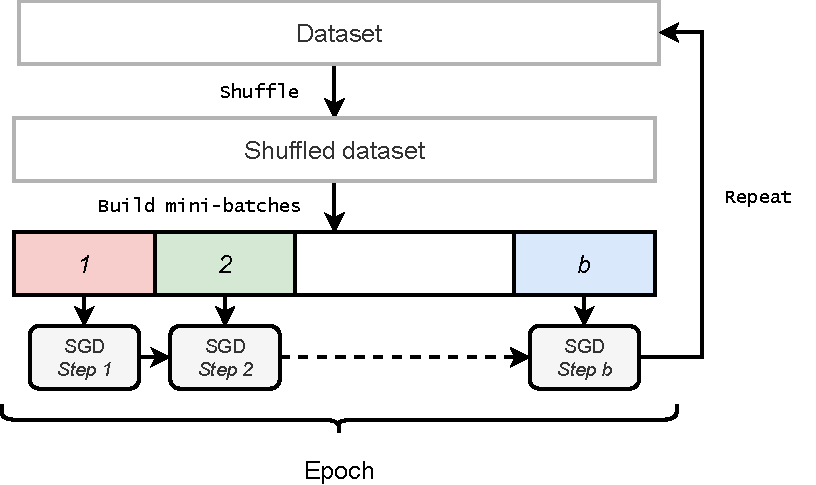
\includegraphics[width=0.7\textwidth]{images/stochastic_optimization.pdf}
    \caption{Building the mini-batch sequence: after shuffling, stochastic optimization starts at mini-batch $1$, which is composed of the first $r$ elements of the dataset. It proceeds in this way to mini-batch $b$ (where $b = \frac{n}{r}$, assuming the dataset size is perfectly divisible by $r$). After one such \textit{epoch}, training proceed with mini-batch $b+1$, which is composed of the first $r$ elements of the shuffled dataset. The second epoch ends at mini-batch $2b$, and so on.}
    \label{fig:building_mini_batches}
\end{figure}

Gradient descent applied on mini-batches of data is an example of \textbf{stochastic gradient descent} (SGD). Due to the properties discussed above, SGD can be proven to converge to a minimum in expectation, and it is the preferred optimization strategy when training differentiable models.

The last remaining issue is how to select the mini-batches. For large datasets, sampling elements at random can be expensive, especially if we need to move them back and forth from the GPU memory. An intermediate solution that lends itself to easier optimization is the following:

\begin{enumerate}
    \item Begin by shuffling the dataset.
    \item Then, subdivide the original dataset into mini-batches of $r$ \textit{consecutive} elements and process each of them sequentially. Assuming a dataset of size $n=rb$, this results in $b$ mini-batches and hence $b$ steps of SGD. If we are executing the code on a GPU, this step includes sending the mini-batch to the GPU memory.
    \item After completing all mini-batches constructed in this way, return to point 1 and iterate.
\end{enumerate}

\begin{mypy}{Building the mini-batch sequence with PyTorch's data loader: all frameworks provide similar tools.}{code:data_loader}
# A dataset composed by two tensors
dataset = torch.utils.data.TensorDataset(
    torch.randn(1000, 3), torch.randn(1000, 1))

# The data loader provides shuffling and mini-batching
dataloader = torch.utils.data.DataLoader(dataset, 
                shuffle=True, batch_size=32)

for xb, yb in dataloader:
  # Iterating over the mini-batch sequence (one epoch)
  # xb has shape (32, 3), yb has shape (32, 1)
\end{mypy}

One complete loop of this process is called an \textbf{epoch} of training, and it is a very common hyper-parameter to specify (e.g., for a dataset of $1000$ elements and mini-batches of $20$ elements, “\textit{training for 5 epochs}” means training for $250$ iterations). The expensive shuffling operation is only done once per epoch, while in-between an epoch mini-batches can be quickly pre-fetched and optimized by the framework. This is shown schematically in Figure \ref{fig:building_mini_batches}. Most frameworks provide a way to organize the dataset into elements that can be individually  indexed, and a separate interface to build the mini-batch sequence. In PyTorch, for example, this is done by the {\footnotesize\mintinline{python}{Dataset}} and {\footnotesize\mintinline{python}{DataLoader}} interfaces, respectively - see Box \ref{code:data_loader}.


\begin{figure}[t]
    \centering
    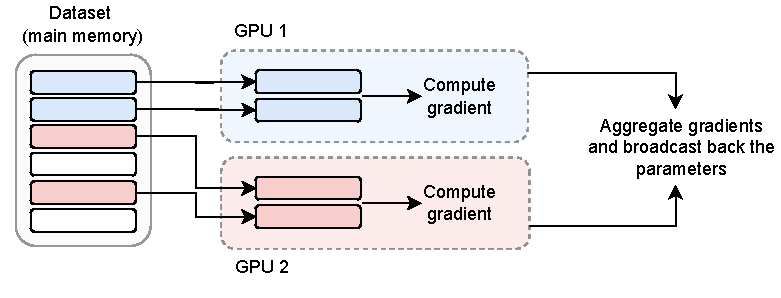
\includegraphics[width=0.75\textwidth]{images/mini_batch.pdf}
    \caption{A simple form of distributed stochastic optimization: we process one mini-batch per available machine or GPU (by replicating the weights on each of them) and sum or average
    the corresponding gradients before broadcasting back the result (which is valid due to the linearity of the gradient operation). This requires a synchronization mechanism across the machines or the GPUs.}
    \label{fig:mini_batch}
\end{figure}

This setup also leads itself to a simple form of parallelism across GPUs or across machines. If we assume each machine is large enough to hold an entire copy of the model's parameters, we can process different mini-batches in parallel over the machines and then sum their local contributions for the final update, which is then broadcasted back to each machine. This is called a \textbf{data parallel} setup in PyTorch,\footnote{\url{https://pytorch.org/tutorials/intermediate/ddp_tutorial.html}} and it is shown visually in Figure \ref{fig:mini_batch}. More complex forms of parallelism, such as \textbf{tensor parallelism}, are also possible, but we do not cover them in this book.


\section{Activation functions}
\label{sec:activation_functions}

We close the chapter by providing a brief overview on the selection of activation functions. As we stated in the previous section, almost any element-wise non-linearity is theoretically valid. However, not all choices have good performance. As an example, consider a simple polynomial function, for some user-defined positive integer $p$:
%
$$
\phi(s)=s^p
$$
%
For large $p$, this will grow rapidly on both sides, compounding across layers and resulting in models which are hard to train and with numerical instabilities. 

Historically, neural networks were introduced as approximate models of biological neurons (hence, the name \textit{artificial NNs}). In this sense, the weights $\mathbf{w}^\top$ in the dot product $\mathbf{w}^\top \mathbf{x}$ were simple models of synapses, the bias $b$ was a threshold, and the neuron was “activated” when the cumulative sum of the inputs surpassed the threshold:
%
$$
s = \mathbf{w}^\top\mathbf{x}-b \;,\; \phi(s)= \mathbb{I}_{s \ge 0}
$$
%
where $\mathbb{I}_{b}$ is an indicator function which is $1$ when $b$ is true, $0$ otherwise. Because this activation function is non-differentiable, the sigmoid $\sigma(s)$ can be used as a soft-approximation. In fact, we can define a generalized sigmoid function with a tunable slope $a$ as $\sigma_a(s) = \sigma(as)$, and we have:
%
$$
\lim_{a \rightarrow \infty}\sigma_a(s)=\mathbb{I}_{s \ge 0}
$$
%
Another common variant was the hyperbolic tangent, which is a scaled version of the sigmoid in $[-1,+1]$:
%
$$
\tanh(s)=2\sigma(s)-1
$$
%
Modern neural networks, popularized by AlexNet in 2012 \cite{krizhevsky2012imagenet}, have instead used the ReLU function in \eqref{eq:relu}. The relative benefits of ReLU with respect to sigmoid-like functions will be discussed in the next chapter. We note here that ReLUs have several counter-intuitive properties. For example, they have a point of non-differentiability in $0$, and they have a large output sparsity since all negative inputs are set to $0$. This second property can result in what is known as “dead neurons”, wherein certain units have a constant $0$ output for all inputs. This can be solved by a simple variant of ReLU, known as \textbf{Leaky ReLU}:
%
\begin{equation}
\text{LeakyReLU}(s) = \begin{cases} s & \text{ if } s \ge 0 \\ \alpha s & \text{ otherwise } \end{cases} 
\label{eq:leaky_relu}
\end{equation}
%
for a very small $\alpha$, e.g., $\alpha = 0.01$. We can also train a different $\alpha$ for each unit (as the function is differentiable with respect to $\alpha$). In this case, we call the AF a \textbf{parametric ReLU} (PReLU) \cite{he2015delving}. Trainable activation functions are, in general, an easy way to add a small amount of flexibility with a minor amount of parameters -- in the case of PReLU, one per neuron.

Fully-differentiable variants of ReLU are also available, such as the \textbf{softplus}:
%
\begin{equation}
\text{softplus}(s)=\log(1+\exp(s))
\label{eq:softplus}
\end{equation}
%
The softplus does not pass through the origin and it is always greater than $0$. Another variant, the \textbf{exponential linear unit} (ELU), preserves the passage at the origin while switching the lower bound to $-1$:
%
\begin{equation}
\text{ELU}(s)=\begin{cases} s & \text{ if } s \ge 0 \\ \exp(s)-1 & \text{ otherwise } \end{cases}
\label{eq:elu}
\end{equation}
%
Yet another class of variants can be defined by noting the similarity of ReLU with the indicator function. We can rewrite the ReLU as:
%
$$
\text{ReLU}(s)=s \mathbb{I}_{s \ge 0}
$$
%
Hence, ReLU is identical to the indicator function on the negative quadrant, while replacing $1$ with $s$ on the positive quadrant. We can generalize this by replacing the indicator function with a weighting factor $\beta(s)$:
%
$$
\text{GeneralizedReLU}(s)=\beta(s)s
$$
%
Choosing $\beta(s)$ as the cumulative Gaussian distribution function, we obtain the \textbf{Gaussian ELU} (GELU) \cite{hendrycks2016gaussian}, while for $\beta(s) = \sigma(s)$ we obtain the \textbf{sigmoid linear unit} (SiLU)  \cite{hendrycks2016gaussian}, also known as the \textbf{Swish} \cite{ramachandran2017searching}. We plot some of these AFs in Figure \ref{fig:activation_functions}. Apart from some minor details (e.g., monotonicity in the negative quadrant), they are all relatively similar, and it is in general very difficult to obtain a significant boost in performance by simply replacing the activation function.

\begin{figure}[t]
    \centering
    \begin{subfigure}[b]{0.18\textwidth}
    \includegraphics[width=\textwidth]{images/activation_function_relu.pdf}
    \caption{ReLU}
    \end{subfigure}
    \hfill
    \begin{subfigure}[b]{0.18\textwidth}
    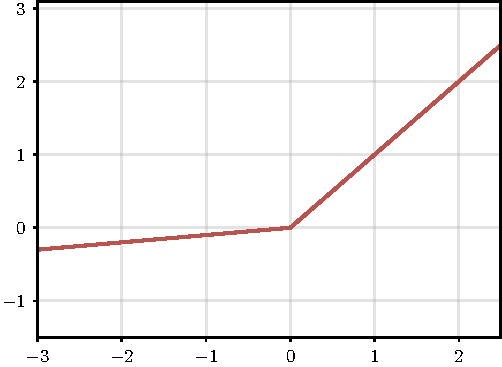
\includegraphics[width=1.0\textwidth]{images/activation_function_LeakyReLU.pdf}
    \caption{LeakyReLU}
    \end{subfigure}
    \hfill
    \begin{subfigure}[b]{0.18\textwidth}
    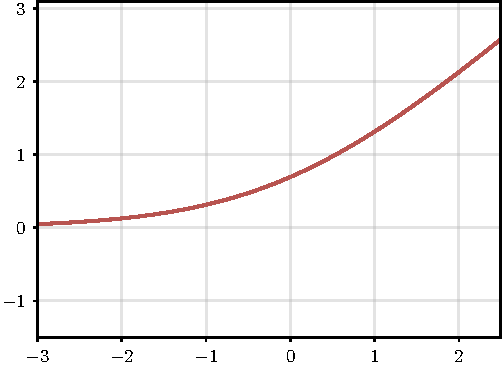
\includegraphics[width=1.0\textwidth]{images/activation_function_Softplus.pdf}
    \caption{Softplus}
    \end{subfigure}
    \hfill
    \begin{subfigure}[b]{0.18\textwidth}
    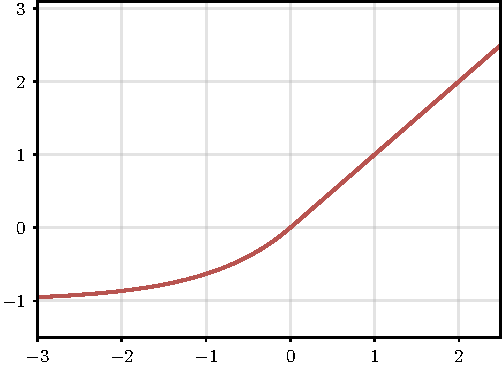
\includegraphics[width=1.0\textwidth]{images/activation_function_ELU.pdf}
    \caption{ELU}
    \end{subfigure}
    \hfill
    \begin{subfigure}[b]{0.18\textwidth}
    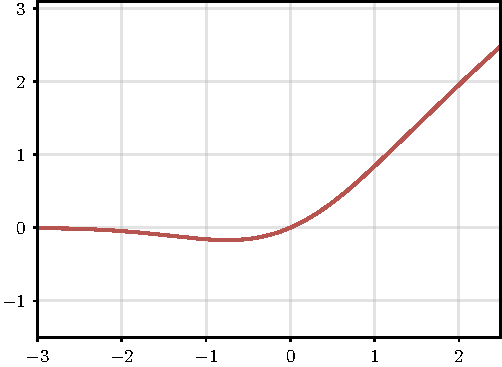
\includegraphics[width=1.0\textwidth]{images/activation_function_GELU.pdf}
    \caption{GELU}
    \end{subfigure}
    \hfill
    \caption{Visual comparison of ReLU and four variants: LeakyReLU \eqref{eq:leaky_relu}, Softplus \eqref{eq:softplus}, ELU \eqref{eq:elu}, and GELU. LeakyReLU is shown with $\alpha=0.1$ for better visualization, but in practice $\alpha$ can be closer to $0$ (e.g., $0.01$)..}
    \label{fig:activation_functions}
\end{figure}

Multiple trainable variants of each function can be obtained by adding trainable parameters to the functions. For example, a common trainable variant of the Swish with four parameters $\left\{a,b,c,d\right\}$ is obtained as:
%
\begin{equation}
\text{Trainable-Swish}(s)=\sigma(as+b)(cs+d)
\label{eq:trainable_swish}
\end{equation}
%
We can also design \textbf{non-parametric} activation functions, in the sense of activation functions that do not have a fixed number of trainable parameters. For example, consider a generic set of (non-trainable) scalar functions $\phi_i$ indexed by an integer $i$. We can build a fully flexible activation function as a linear combination of $n$ such bases:
%
\begin{equation}
\phi(s) = \sum_{i=1}^n \alpha_i \phi_i(s) \,
\label{eq:non_parametric_af}
\end{equation}
%
where $n$ is an hyper-parameter, while the coefficients $\alpha_i$ are trained by gradient descent. They can be the same for all functions, or different for each layer and/or neuron. Based on the choice of $\phi_i$ we obtain different classes of functions: if each $\phi_i$ is a ReLU we obtain the \textbf{adaptive piecewise linear} (APL) function \cite{agostinelli2014learning}, while for more general kernels we obtain the \textbf{kernel activation function} (KAF) \cite{marra2018learning,scardapane2019kafnets}. Even more general models can be obtained by considering functions with multiple inputs and multiple outputs \cite{li2023generalized}. See \cite{apicella2021survey} for a survey.

In general, there is no answer to the question of “what is the best AF”, as it depends on the specific problem, dataset, and architecture. Apart from its performance, ReLU is a common choice also because highly optimized code kernels are available and it adds a minor cost overhead. It is important to consider the fundamental computational trade-off that, for a given budget, more complex AFs can result in having smaller width or smaller depth, potentially hindering the performance of the entire architecture. For this reason, AFs with a lot of trainable parameters are less common.

\begin{supportbox}{Design variants}
Not every layer fits into the framework of \textit{linear projections} and \textit{element-wise} non-linearities. For example, the \textbf{gated linear unit} (GLU) \cite{dauphin2017language} combines the structure of \eqref{eq:trainable_swish} with multiplicative (Hadamard) interactions:
%
\begin{equation}
f(\mathbf{x}) = \sigma\left(\mathbf{W}_1\mathbf{x}\right)\odot\left(\mathbf{W}_2\mathbf{x}\right)
\label{eq:glu}
\end{equation}
%
where $\mathbf{W}_1$ and $\mathbf{W}_2$ are trained. Another common variant, the SwiGLU, replaces the sigmoid in \eqref{eq:glu} with a Swish function \cite{shazeer2020glu}. In a \textbf{maxout} network \cite{goodfellow2013maxout} each unit produces the maximum of $k$ (hyper-parameter) different projections. Replacing the linear projection $\mathbf{W}$ with a matrix of trainable non-linearities $W_{ij} \rightarrow \phi_{ij}(x_j)$ of the form \eqref{eq:non_parametric_af} has also been proposed recently under the name of \textbf{Kolmogorov-Arnold networks} (KAN, \cite{liu2024kan}).
%
\end{supportbox}

\section*{From theory to practice}

\begin{wrapfigure}{r}{3.0cm}
\vspace{-3em}
\includegraphics[width=3.0cm]{images/shutterstock_2075221579.jpg}
\vspace{-5em}
\end{wrapfigure}

This chapter has introduced two key requirements for any general-purpose framework for training differentiable models:

\begin{enumerate}
\item A way to handle large datasets that need to be shuffled, separated into mini-batches, and moved back and forth from the GPU. In PyTorch, most of this is implemented via the {\mintinline{python}{Dataset}} and \mintinline{python}{DataLoader} interfaces, as in Box \ref{code:data_loader}.\footnote{\url{https://pytorch.org/tutorials/beginner/basics/data_tutorial.html}}
\end{enumerate}

\begin{enumerate}\addtocounter{enumi}{1}
\item A mechanism to build models from the combination of basic blocks, known as \textit{layers}. In PyTorch, layers are implemented in the \mintinline{python}{torch.nn} module, and they can be composed via the \mintinline{python}{Sequential} interface or by subclassing the \mintinline{python}{Module} class, as in Box \ref{code:fully_connected_layer}.
\end{enumerate}

I suggest you now try to replicate one of the many quick guides available on the documentation of PyTorch.\footnote{\url{https://pytorch.org/tutorials/beginner/basics/quickstart_tutorial.html}} Everything should be reasonably clear, apart from the gradient computation mechanism, introduced in the next chapter. This is also a good time to investigate HuggingFace Datasets, which combines a vast repository of datasets with an interface to process and cache them which is framework-agnostic and backed by Apache Arrow.\footnote{\url{https://huggingface.co/docs/datasets/en/quickstart}}

JAX does not provide high-level utilities. For data loading you can use any existing tool, including PyTorch's data loaders and HuggingFace Datasets. For building models, the easiest way is to rely on an external library. Because JAX is fully functional, object-oriented abstractions like Box \ref{code:fully_connected_layer} are not possible. My personal suggestion is Equinox \cite{kidger2021equinox}, which provides a class-like experience by combining the basic data structure of JAX (the \mintinline{python}{pytree}) with callable nodes.